
\documentclass[tikz,border=7pt]{standalone}
\usepackage[utf8]{inputenc}
\usepackage[T1]{fontenc}
\usepackage{amsmath}
\usepackage{xcolor}
\usetikzlibrary{arrows.meta,calc,angles,quotes,patterns,positioning}
\definecolor{brand}{HTML}{1E3A8A}
\definecolor{brandtwo}{HTML}{2563EB}
\definecolor{accentred}{HTML}{EF4444}
\definecolor{accentgreen}{HTML}{16A34A}
\definecolor{accentorange}{HTML}{F59E0B}
\definecolor{muted}{HTML}{64748B}
\definecolor{lightblue}{HTML}{EEF6FF}
\tikzset{force/.style={-{Latex[length=3mm]}, line width=1.15pt}, axis/.style={-{Latex[length=2mm]}, line width=.8pt, color=muted}, body/.style={draw=brandtwo, fill=lightblue, line width=1pt, rounded corners=2pt}, lab/.style={font=\small, text=brand}, sml/.style={font=\scriptsize, text=muted}}
\begin{document}

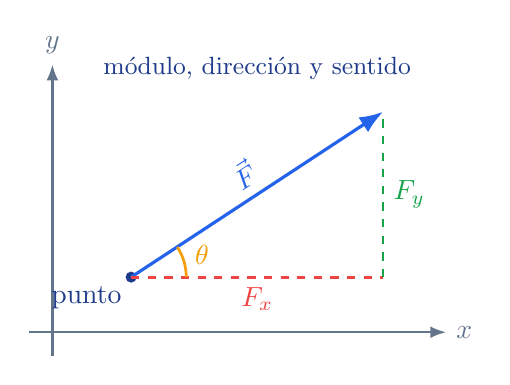
\begin{tikzpicture}[scale=1]
\draw[axis] (-.3,0)--(5,0) node[right] {$x$}; \draw[axis] (0,-.3)--(0,3.4) node[above] {$y$};
\fill[brand] (1,.7) circle (2pt) node[below left, text=brand] {punto};
\draw[force, color=brandtwo] (1,.7)--(4.2,2.8) node[midway,above,sloped] {$\vec F$};
\draw[dashed, color=accentred, line width=1pt] (1,.7)--(4.2,.7) node[midway,below] {$F_x$};
\draw[dashed, color=accentgreen, line width=1pt] (4.2,.7)--(4.2,2.8) node[midway,right] {$F_y$};
\draw[accentorange, line width=1pt] (1.7,.7) arc[start angle=0,end angle=33,radius=.7]; \node[text=accentorange] at (1.9,.98) {$\theta$};
\node[align=center, lab] at (2.6,3.35) {módulo, dirección y sentido};
\end{tikzpicture}

\end{document}